\documentclass[]{article}
\usepackage[pdftex]{graphicx}  
\begin{document}

\begin{enumerate}

\item Figure \ref{dogigree} is a pedigree of miniature schnauzers (a dog breed). Female \#2 has already had one litter, and male \#3 has already sired two offspring with female \#4. A breeder is interested in mating female \#2 and male \#3, but is worried about a recessive X-linked disorder called Von-Willibrands disease in their offspring. Answer the following:

\begin{enumerate}
\item What are the genotypes of dogs \#1, \#3, and \#4? (4pts)
\item The breeder had female \#2 tested for the disease, and the test result suggested she was a carrier. The test is imperfect, however, and ~20\% of the time returns an incorrect positive result. You are a geneticist brought in to advise the breeder. What is the most likely genotype of dog \#2? Explain how you reach this conclusion. (4pts)
\item Given the genotypes above, what is the probability that dogs \#2 and \#3 will have: (2 pts)
\begin{enumerate}
\item A male puppy with Von-Willibrands disease?
\item A female puppy with Von-Willibrands disease?
\item A normal female puppy?
\item A normal male puppy?
\end{enumerate}
\end{enumerate}

%-------------------------------------------------------------------
\begin{figure*}[h]
  \begin{center}
   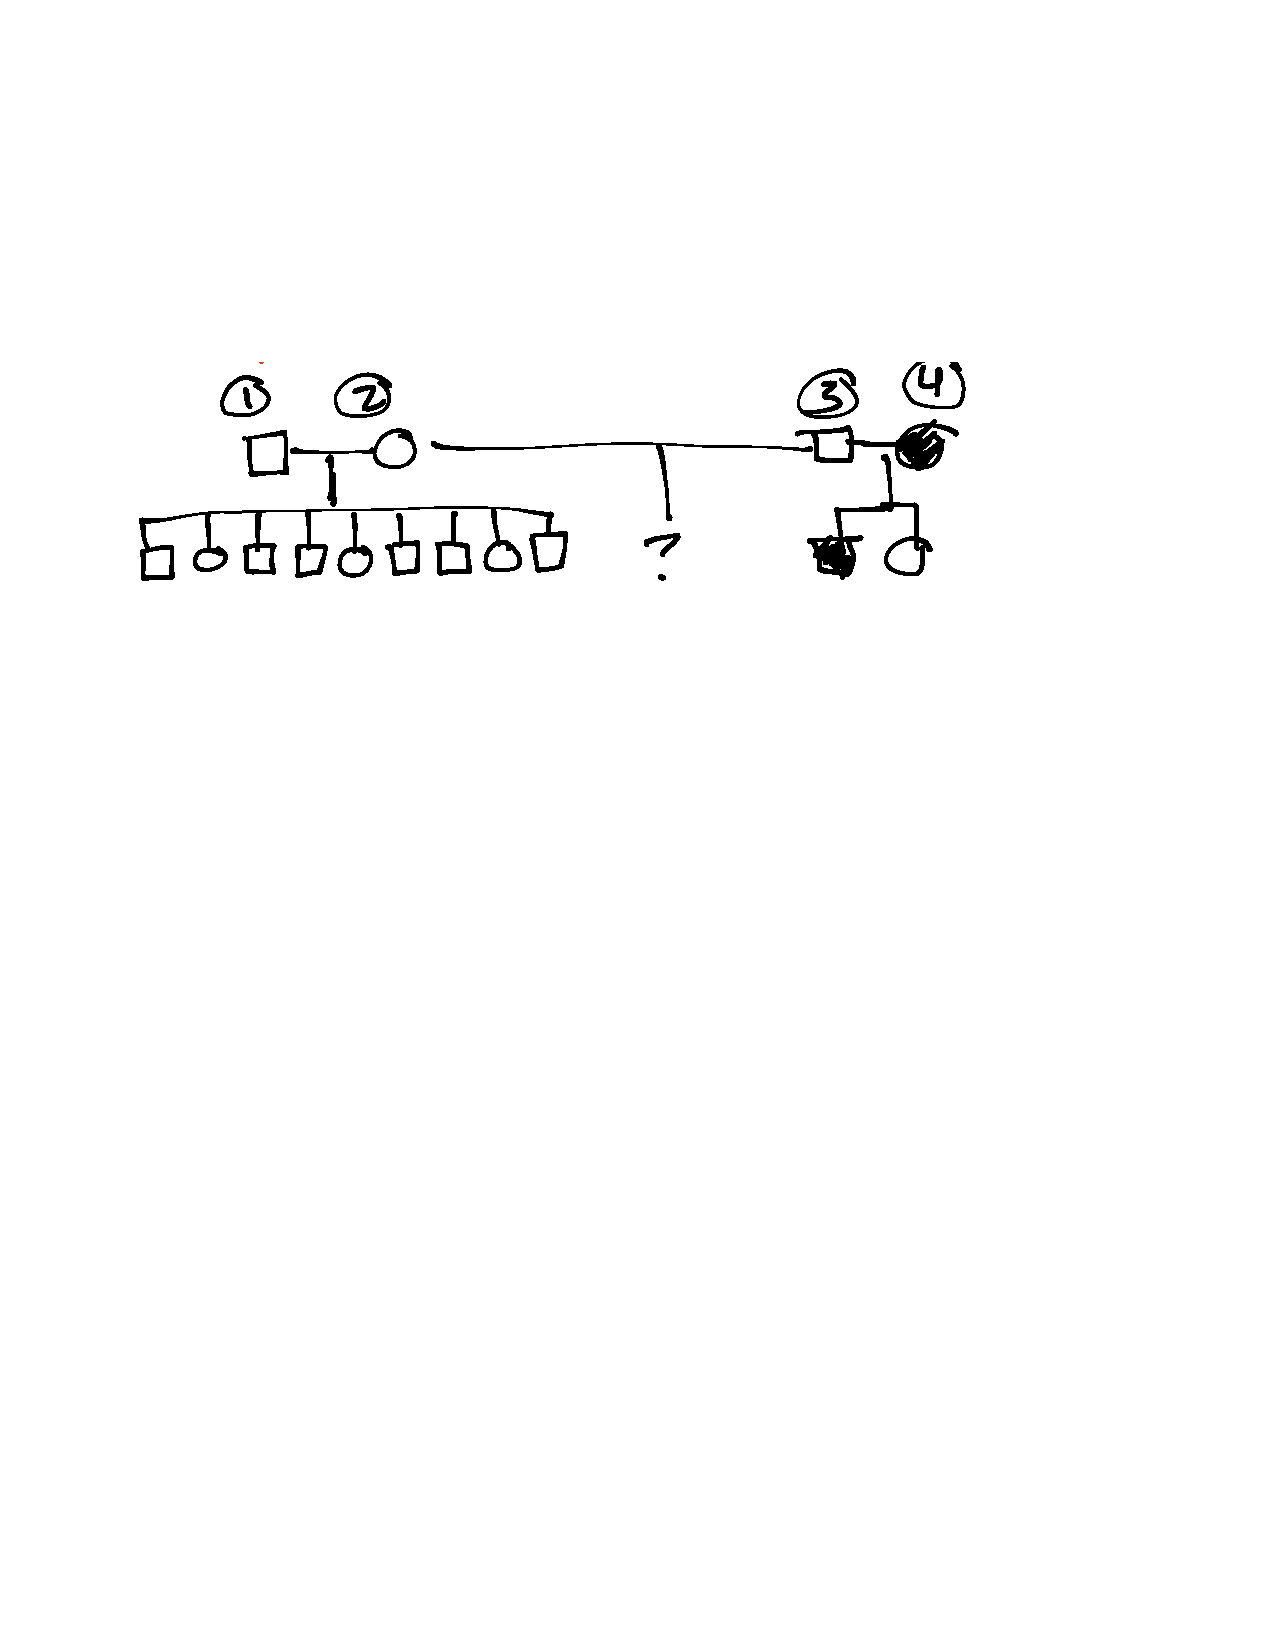
\includegraphics[width=130mm]{/Users/jri/src/bis101/images/pedigree_test.pdf}
\caption{A pedigree of miniature schnauzers. Filled symbols (square=male, circle=female) represent dogs with Von-Willibrands disease. Empty symbols are dogs with wild-type phenotypes.}
\label{dogigree}
  \end{center}
\end{figure*}
%-------------------------------------------------------------------

\item You are interested in understanding the genetics of furriness in rabbits. You recruit 18 rabbit owners to bring in their bunnies for measurement.  Each bunny's fluffiness is measured on a scale of 1 (no hair) to 10 (maximum fluffy). Phenotypes for all 18 bunnies are shown in Table \ref{fluffy}. 

\begin{enumerate}
\item Calculate the phenotypic variance for fluffiness (4 pts).
\item In a separate study, you measure the fluffiness of a set of identical rabbit quadruplets that were sold by a breeder to 4 different families.  Their phenotypes are shown in Table \ref{clones}. Using these data, calculate the broad sense heritability of fluffiness in rabbits (6 pts).
\end{enumerate}

\begin{table}[h!]
\caption[]{Rabbit phenotypes.}
\begin{center}
\begin{tabular}{ll}
Rabbit Name & Fluffiness \\  \hline
Baby & 2\\
Baggins & 8\\
Bambi & 9\\
Barbie & 10\\
Basil & 7\\
Bella & 2\\
Benny & 7\\
Big Boy & 5\\
Big-Ears & 2\\
Binky & 10\\
Bluebell & 8\\
Boo Boo & 8\\
Buddy & 4\\
Bugs & 4\\
Bun Bun & 4\\
Bunnicula & 3\\
Bunzilla & 6\\
Buttercup & 4\\
\end{tabular}
\end{center}
\label{fluffy}
\end{table}

\begin{table}[h!]
\caption[]{Quadruplet rabbit phenotypes.}
\begin{center}
\begin{tabular}{ll}
Rabbit Name & Fluffiness \\  \hline
Oliver & 7\\
Ollie & 8\\
Oreo & 9\\
Oscar & 9\\
\end{tabular}
\end{center}
\label{clones}
\end{table}

\item Abscisic acid is an important regulator of seed maturation and germination in plants. You have two mutant maize plants that make insufficient levels of abscisic acid and thus their kernels germinate prematurely on the cob. When you self the first mutant it produces 214 mutants and 70 wild-type offspring.  When you self the second mutant it produces 345 mutant offspring. When you cross the two mutants they produce 265 mutant and 272 wild-type offspring. Draw the genotypes of both mutant lines, indicating the number of loci and the dominance of the alleles involved (10pts).

\item The following two questions refer to the paper by Schempske and Bradshaw (1999). 
\begin{enumerate}
\item Briefly describe one surprising conclusion that Schempske and Bradshaw found in their analysis of pollinator preferences in \emph{Mimulus}. (5pts)
\item Carotenoid content in \emph{Mimulus} flowers is controlled by a single Mendelian locus called \emph{yup}. At this locus the \emph{M. cardinalis} allele is recessive to the \emph{M. lewissii} allele. In a population of F2 plants generated from a cross between \emph{M. lewissii}  and \emph{M. cardinalis}, provide an estimate and an explanation as to what you think the broad sense heritability for flower color would be (\emph{hint: no calculations are needed to answer this question})(5 pts).
\end{enumerate}


\item Liu



\item Johnston

\item Genetic mapping

\item Ibarra-Laclette 

\item Genomics/phylogenetics

\item Chromosomal evolution

\end{enumerate}

\end{document}